 \section{Hardware}
 \fxnote{der skal laves referecener og generelt skrives mere dybdegående spec beskrivelse}
%metatekst til hardware
 Dette afsnit indeholder alt omkring hardware delene, fra hvilke krav der er gået ud fra til hvad der er fundet frem til. Denne blok beskriver forbindelserne mellem diverse hardware med et internal block definition diagram. Dette diagram er med til at sikre at delene kan kommunikere sammen, uden unødvendige adaptere og omformere. Yderligere er der beskrevet hvordan information søgning, og viden er fundet omkring komponenterne. Primær kan det siges at hardware delene er fundet på Ebay.com(kilder til de konkrete sider?(måske under hvert produkt?)), for at hold budgettet i bund. Den manglende datablade og lidt tvivlsomme kvalitet er accepteret, da dette projekt først og fremmest er  ”\textit{proof of concept}” projekt.
 
\subsection{Block Definition Diagram} 

\begin{figure}[H]
	\centering
	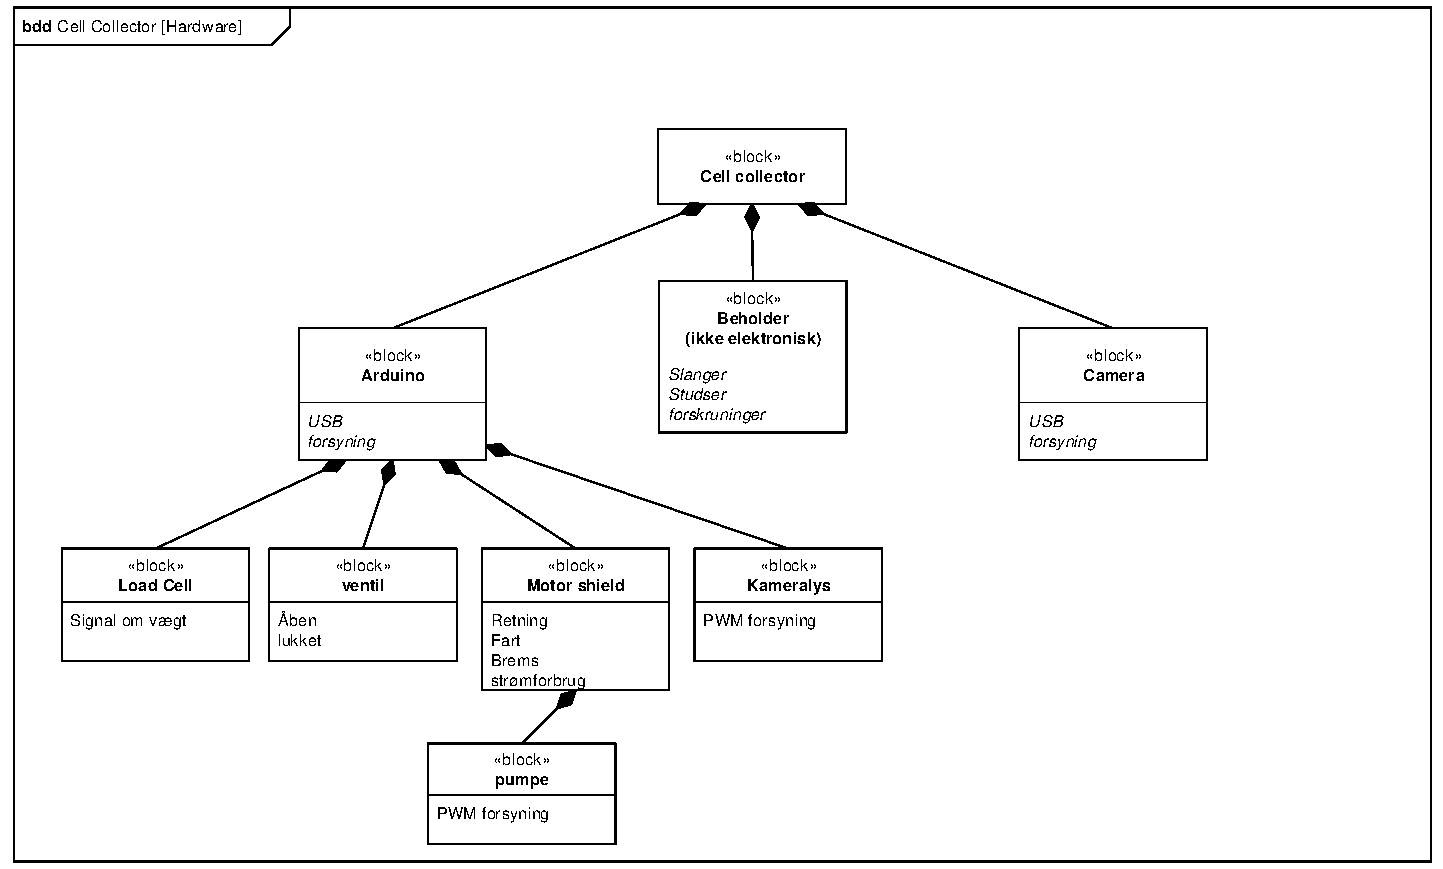
\includegraphics[width=1\textwidth]{pdf/BDD_Hardware_cropped.pdf}
	\caption{BDD - Cell Collector [Hardware]}
	\label{fig:bdd_Hardware}
\end{figure}

\subsection{internal block Diagram} 
\begin{figure}[H]
	\centering
	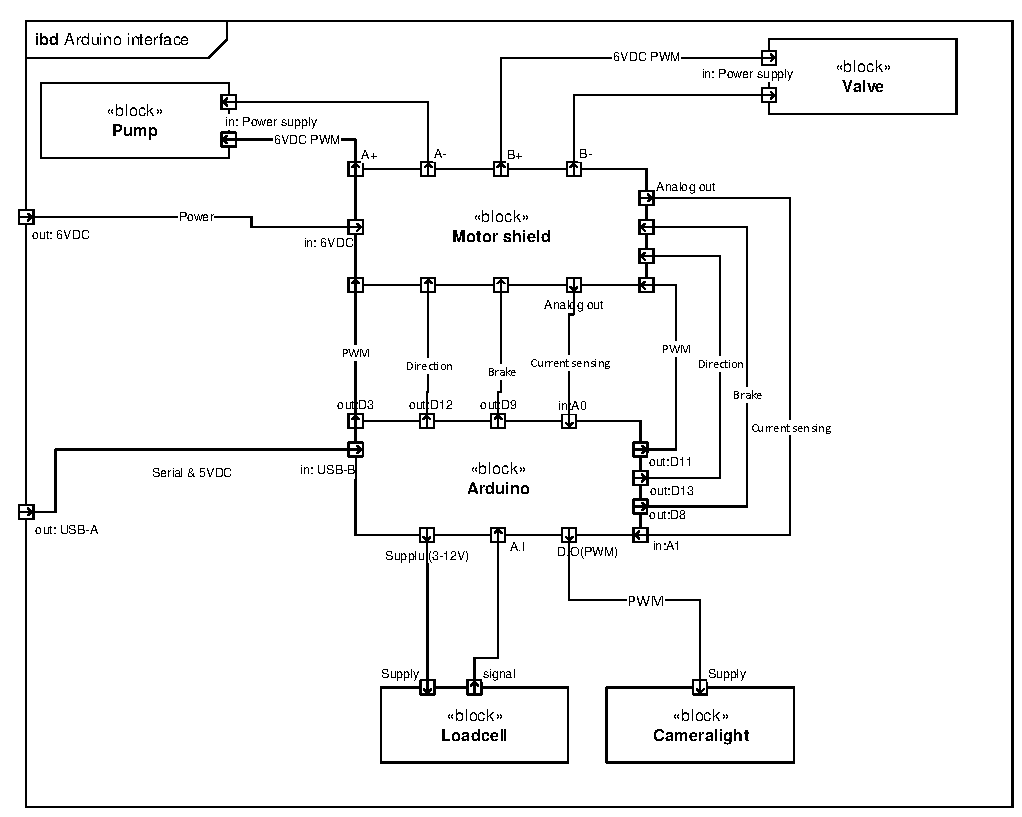
\includegraphics[width=1\textwidth]{pdf/IBD_Hardware(Arduino)_cropped.pdf}
	\caption{IBD - Cell Collector [Hardware]}
	\label{fig:ibd_Hardware}
\end{figure}



\subsection{Kamera}
Kameraet skal detektere de langerhanske øer, når de kommer forbi i slangen.  Da de langerhanske øer skiller sig ud på den måde at de er mere lyse end resten af vævet, er det underordnet om kameraet er et farve kamera. Da systemet ikke skal operere under en stor hastighed er et standard frame rate valgt, 30f/s. Kameraet opløsning er valgt ud fra, at det skal kunne se de langerhanske øer med en størrelse på 100-300um. Til bestemmelse til dette er der brugt følgende formel:
 
for at kameraet har mulighed for at se lidt flere detaljer og forhåbning om at det kan være tættere på end 10 cm, er det besluttet er et 2 megapixels kamera burde være passende.

\url{http://www.baslerweb.com/media/documents/BAS1408_White_paper_Camera_Selection_EN.pdf}


Da kameraet er en elementær del af systemet opsætning, blev det besluttet at købe det ved en mere pålidelig forhandler til en overkommelig pris. Farnell


\url{http://dk.farnell.com/duratool/bw788/microscope-digital-usb-25x-200x/dp/2319420}
 
 \subsection{Slanger}
slangerne skal bruges til at føre opløsningen med de langerhanske øer, i gennem systemet bla. forbi kameraet. Da de største langerhanske øer, som systemet skal kunne klare er 300um er der valgt at slangerne skal have en indre diameter på cirka 500um. Yderligere har et krav været at kameraet skal kunne se igennem slangerne, derfor er der tilkøbt et glasrør som kameraet kan se igennem. Grundet besvar med at finde forhandler til de små mængder skal skal bruge til projektet, er der skabt kontakt til Mikrolab. Som har været en stor hjælp med at finde dele til slanger mm.

\subsection{Arduino}
Arduino er en open source platform til fremstilling af prototype print, som kan bruge til at styre forskellige systemer som dette. Det er valgt at bruge en arduino som controller for at spare tid, i forhold til selv at lave et print med en microcontroller. Samt er dette et udviklingskort der er brugt i et stort omfang omkring i verden. Derfor er det en platform der er nemt tilgængelig og forholdsvis prisvenlig. Da det som sagt er en open source platform, kan der købes forskellige versioner. Microcontrolleren der sidder på denne version er et gruppen har brugt, og arbejdet med til et tidligere projekt. Hvilket også betyder at den allerede er i gruppen beholdning af produkter.
Arduinoen skal bruges til at styre pumpe ved hjælp af ”mini motor drive shield”, det skal køres der igennem for at være sikker på at der leveres effekt nok til pumpen. Yderligere har det den fordel at strømmen til pumpen kan måles og at den er galvanisk adskilt fra forsyningen til arduinoen. Dette er dog ikke arduinoen eneste opgave den skal blandt andet også styre ventilen til sortering og lyset til kameraet.

\subsection{Ventil}
Ventilens funktion er at sorterer de langerhanske øer, fra resten af opløsningen. Der findes utrolig mange typer af ventiler, med et store prisforskelle. Ventilen er en vigtig del af systemets hardware, det er svært at finde ventiler med 500um studser. Det kan god lade sig gøre at få adaptere så større ventiler kan bruges, men sporbarheden omkring hvor den enkelte ø befinder sig, bliver svært hvis kammeret pludseligt bliver stort. Dette er et stykke hardware, hvor der kan bruges meget tid og mange penge.
Kravene til ventilen er at den skal være 3vejs 1 tilgang og 2 udgange, yderligere skal studserne kunne tilpasses slange størrelsen, være til væske og have en lukke/åbne tid under 50ms.

\subsection{Pumpe}
Pumpen skal skabe det nødvendige flow i væsken fra det ene punkt til det andet, flowet skal være lavt nok til at kameraet kan nå at detekterer en ø. Hvilket gør at en variable hastighed vil være optimal. Der findes mange forskellige typer stempel pumper, peristaltiske pumper og vakuum pumper er et udsnit af dem der er blevet kigget på. Ligesom ved ventilen er det også et produkt der kan få budgettet til at skride, derfor er der igen gået på kompromis og brug ebay forhandlere som leverandører. Der er bestilt en peristaltisk pumpe som virker ved at klemme på slangen og derved skabe et flow, det er dog uvist hvordan de langerhanske øer vil opfører sig ved sådan en pumpe. Der er også købt en vakuum pumpe, som muligvis kan sidde efter ventilen. Der skal dog stadig skabes et flow til de sorterede øers beholder, måske en kombination vil være det optimale. En modultest af de enkelte pumper skal afgøre hvilken løsning der er den mest optimale. 
vakuumpumper:
\subsubsection{Vakuumpumper}
\url{ http://www.ebay.com/itm/281571300037}

\url{http://www.ebay.com/itm/161665897119?_trksid=p2054502.m570.l4467&_trkparms=gh1g%3DI161665897119.N19.S2.M-4218.R1.TR2}

\subsubsection{Peristaltiskepumper}

\url{http://www.ebay.com/itm/6V-Peristaltic-Pump-Dosing-Water-Pump-DC-Motor-Tube-For-Aquarium-Lab-Analytical-/131367703927?hash=item1e96201577}

\subsection{Beholdere}
Systemet består af tre beholdere der hver i især har sin egen funktion. Den første kaldes celleopløsningbeholderen, som skal indeholde den usorteret opløsning med de langerhanske øer. Beholder nummer to kaldes isolerede langerhanske øer beholderen, som er den beholder hvor de isolerede øer samles i. Den tredje beholder er waste beholderen, den skal have resten af opløsningen som ikke består af langerhanske øer. størrelses Kravene til beholderne er som at opløsningsbeholderen skal mindst være 250ml, da det er den største tænkelige opløsningen der vil blive brugt. Wastebeholderen skal således være dobbelt så stor, så der kan køres to sorterings cyklusser uden at skulle tømme beholderen i mellem. Den isolerede beholder, skal blot kunne rumme mængden af de isolerede øer. Da projektet som tidligere nævnt er et ”prove og concept” er den eneste beholder der er hentet informationer om, opløsningsbeholderen. Den bør være støvtæt, uden at være lufttæt da der ellers vil dannes et vakuum i beholderen. Derudover vil det være en fordel hvis den er forholdsvis robust, så den kan køles ned osv. på et senere tidspunkt.

\subsection{Loadcell}
Loadcellen eller vægtcellen som det kan kaldes på dansk, skal bruges det er kontroller om der er væske i celleopløsningsbeholderen. Det vil sige hvs operatøren ikke har fyldt noge ti beholderen, kan der gives en systembesked omkring dette. Det mest optimale er at der hele tiden er væske i slangerne i systemet, det er det vægtcellen skal hjælpe med. Den indkøbte vægtcellen kan veje op til et kg

\url{http://www.ebay.com/itm/281311660424}


